\documentclass[aspectratio=169]{beamer}

\mode<presentation>
\usetheme{Boadilla}
\definecolor{redback}{RGB}{140,0,0}
\definecolor{blue}{RGB}{30,90,205}
\definecolor{red}{RGB}{213,94,0}
\definecolor{green}{RGB}{0,128,0}
\setbeamercolor{title}{fg=redback}
\setbeamercolor{frametitle}{fg=redback}
\setbeamercolor{block title}{bg=redback, fg=white}
\setbeamercolor{block body}{bg=white}
\setbeamercolor{structure}{fg=redback}
\setbeamercolor{item projected}{fg=white}
\setbeamercolor{item}{fg=redback}
\setbeamercolor{subitem}{fg=redback}
\setbeamercolor{section in toc}{fg=redback}
\setbeamercolor{description item}{fg=redback}
\setbeamercolor{caption name}{fg=redback}
\setbeamercolor{button}{bg=redback, fg=white}
\setbeamercolor{caption name}{fg=redback}
\usepackage{graphics}
\usepackage{tikz}
\usepackage{amsmath}
\usepackage{bbm}
\usetikzlibrary{decorations.pathreplacing}
\usepackage{geometry}
\usepackage{booktabs}
\usepackage{multirow, makecell}
\usepackage{float}
\usepackage{fancyvrb}
\usepackage{kotex}
\usepackage{caption}
\usepackage{subcaption}
\usepackage{adjustbox}
\usepackage{hyperref}
\usepackage{threeparttable}
\usepackage[scaled=0.92]{helvet}
\usepackage[default]{lato} %If I want a twist
\newenvironment{wideitemize}{\itemize\addtolength{\itemsep}{10pt}}{\enditemize}
\newenvironment{wideenumerate}{\enumerate\addtolength{\itemsep}{10pt}}{\endenumerate}
\newenvironment{widedescription}{\description\addtolength{\itemsep}{10pt}}{\enddescription}
\hypersetup{
colorlinks=true,
linkcolor=redback,
filecolor=green, 
urlcolor=blue,
}
\beamertemplatenavigationsymbolsempty
\setbeamercolor{author in head/foot}{bg=white, fg=redback}
\setbeamercolor{title in head/foot}{bg=white, fg=redback}
\setbeamercolor{date in head/foot}{bg=white, fg=redback}
\setbeamercolor{section in head/foot}{bg=white, fg=redback}
\setbeamercolor{page number in head/foot}{bg=white, fg=redback}
\setbeamercolor{headline}{bg=redback}
\setbeamertemplate{footline}{
    \leavevmode%
    \hbox{%
        \begin{beamercolorbox}[wd=.333333\paperwidth,ht=2.25ex,dp=1ex,center]{date in head/foot}%
            \usebeamerfont{date in head/foot}\insertshortdate
        \end{beamercolorbox}%
        \begin{beamercolorbox}[wd=.444444\paperwidth,ht=2.25ex,dp=1ex,center]{title in head/foot}%
            \usebeamerfont{title in head/foot}\insertshorttitle
        \end{beamercolorbox}%
        \begin{beamercolorbox}[wd=.222222\paperwidth,ht=2.25ex,dp=1ex,center]{page number in head/foot}%
            \usebeamerfont{page number in head/foot} \insertframenumber{} / \inserttotalframenumber
        \end{beamercolorbox}}%
        \vskip0pt%
    }

\setbeamertemplate{section in toc}[sections numbered]
\setbeamertemplate{subsection in toc}{\leavevmode\leftskip=3em\rlap{\hskip-1.75em\inserttocsectionnumber.\inserttocsubsectionnumber}\inserttocsubsection\par}
\setbeamerfont{subsection in toc}{size=\footnotesize}

\newenvironment{transitionframe}{\setbeamercolor{background canvas}{bg=redback}\setbeamertemplate{footline}{} \begin{frame}}{\end{frame}}
\newcommand{\ROM}[1]
    {\MakeUppercase{\romannumeral #1}}
    \DeclareMathOperator*{\plim}{plim}
\makeatletter
\let\@@magyar@captionfix\relax
\makeatother


\title[Recitation 12 (Intro to Econometrics \ROM{2})]{Recitation 12: Regression discontinuity and gradient descent} % Change this regularly
\author[]{Seung-hun Lee }
\institute[]{Columbia University \\ Introduction to Econometrics \ROM{2} Recitation}

\date[April 25th, 2022]{April 25th, 2022}

\begin{document}
\begin{frame}
\titlepage
\end{frame}


%%% Color slides for section headers: Use for colloquium version (The ones bewteen \iffals and \fi)

\begin{transitionframe}
  \begin{center}
         { \Huge \textcolor{white}{Regression discontinuity design}}
       \end{center}
\end{transitionframe}

\begin{frame}
\frametitle{RD tries to achieve `as good as random' without IVs}
\begin{itemize}
\item Finding an instrumental variable $Z_i$ that satisfies relevance, exclusion, and monotonicity might be difficult
\item So what about comparing the entities that barely made the treatment against those who barely missed out? Doable if there is a cutoff
\begin{itemize}
\item Means-tested social program, distance, winning margin, or test score cutoffs
\end{itemize} 
\item RD leverages these cutoffs, with the presumption that individuals around the cutoff are otherwise equal and thus the treatment assignment is as good as random
\item Key difference
\begin{itemize}
\item Less emphasis on overlap condition (unlike CIA)
\item Continuity of the covariates around the cutoff (so we have `as good as random')
\end{itemize}
\end{itemize}
\end{frame}


\begin{frame}
\frametitle{RD as a potential outcome framework: Sharp RDD}
\begin{itemize}
\item \textbf{Sharp RDD}: The assignment into the treatment is binary and determined by
\begin{align*}
D_i=\mathbb{I}(Z_i\geq c(W_i))
\end{align*}
\begin{itemize}
\item $Z_i$ is a running variable that determines cutoffs
\item  $c(W_i)$ can be a known function of $W_i$ or just a constant
\item Everyone above (below) cutoff is treated (not treated)
\end{itemize}
\item Potential outcome framework
\begin{align*}
y_i& = D_iy_i(1)+(1-D_i)y_i(0)\\
&=y_i(0)+D_i(y_i(1)-y_i(0))\\
&=y_i(0)+\mathbb{I}(Z_i\geq c(W_i))\cdot(y_i(1)-y_i(0))
\end{align*}
\item Regression framework: $y_i(d)=\mu(W_i,Z_i,d)+\epsilon_i(d)$
\end{itemize}
\end{frame}

\begin{frame}
\frametitle{RD as a potential outcome framework: Fuzzy RDD}
\begin{itemize}
\item \textbf{Fuzzy RDD}: Allows jump in the probability of being treated $\Pr(D_i|W_i, Z_i)$ at $Z_i=c(W_i)$ that is not necessarily 0 to 1
\begin{itemize}
\item Cases include special exceptions on ineligible and noncompliant treated individuals
\item Sharp RDD is a very special case of fuzzy RDD
\end{itemize}
\item Potential outcomes: The end result is 
\begin{align*}
y_i& = D_iy_i(1)+(1-D_i)y_i(0)\\
&=y_i(0)+D_i(y_i(1)-y_i(0))\\
&=y_i(0)+\Pr(D_i=1|W_i, Z_i=c^*)\cdot(y_i(1)-y_i(0))
\end{align*}
\begin{itemize}
\item $c^*$ is $c^+$ for intended compliers and $c^-$ for ineligibles
\end{itemize}
\end{itemize}
\end{frame}


\begin{frame}
\frametitle{Key is continuity of covariates around the cutoff}
\begin{itemize}
\item  If $Z_i$ has a known cutoff at $c$, we assume that $E[y_i(1)|W_i, Z_i]$ and $E[y_i(0)|W_i, Z_i]$ are continuous around $Z_i=c$. Put if differently, 
\[
E[y_i(d)|W_i, Z_i=c^+]=E[y_i(d)|W_i, Z_i=c^-] \  \text{for each } d\in\{0,1\}
\]
This also implies that the distribution of $(\mu_i(W_i, Z_i,0),\mu(W_i, Z_i,1))$ and $(\epsilon_i(0),\epsilon_i(1))$ is continuous at $Z_i=c$
\item This is to ensure that those who are treated and untreated are observationally equivalent, at least around the cutoff
\item Violation implies an incorrect TE estimate or bunching of certain individuals at the cutoff (bunching)
\begin{itemize}
\item The latter can be tested with McCrary test (for continuous running variables)
\end{itemize}
\end{itemize}
\end{frame}

\begin{frame}
\frametitle{With sharp RD, we identify ATE for $i$'s around the cutoff}
\begin{itemize}
\item For a constant cutoff $c(W_i)=c$, write 
\begin{align*}
E[y_i|W_i, Z_i]&=E[y_i(0)|W_i, Z_i]+E[(y_i(1)-y_i(0))\mathbb{I}(Z_i\geq c)|W_i, Z_i]
\end{align*}
\item These values are different for $Z_i=c^+$ and $c^-$
\begin{align*}
E[y_i|W_i, Z_i=c^+]&=E[y_i(0)|W_i, Z_i=c^+]+E[y_i(1)-y_i(0)|W_i, Z_i=c^+]\\
E[y_i|W_i, Z_i=c^-]&=E[y_i(0)|W_i, Z_i=c^-]
\end{align*}
\item Subtract the two terms 
\begin{align*}
E[y_i|W_i, Z_i=c^+] - E[y_i|W_i, Z_i=c^-]&=E[y_i(0)|W_i, Z_i=c^+]-E[y_i(0)|W_i, Z_i=c^-]\\
 &\ \ \ \ +E[(y_i(1)-y_i(0))|W_i, Z_i=c^+]\\
 &=E[(y_i(1)-y_i(0))|W_i, Z_i=c^+]
\end{align*}
where $E[y_i(0)|W_i, Z_i=c^+]=E[y_i(0)|W_i, Z_i=c^-]$ by continuity assumption
\end{itemize}
\end{frame}

\begin{frame}
\frametitle{With sharp RD, we identify ATE for $i$'s around the cutoff}
\begin{itemize}
\item Again, using continuity assumptions, we get 
\[
E[y_i(1)-y_i(0)|W_i, Z_i=c^+]=E[y_i(1)-y_i(0)|W_i, Z_i=c]
\]
\item Therefore, we have 
\[
E[y_i(1)-y_i(0)|W_i, Z_i=c]=E[y_i|W_i, Z_i=c^+] - E[y_i|W_i, Z_i=c^-]
\]
\item Values of $c^+$ and $c^-$: $[c-h,c+h]$ from optimizing tradeoff between bias and variance
\begin{itemize}
\item Narrow bandwidth: Increases accuracy at the cost of increased variance (vice versa)
\item Very limited external validity: What about people outside of the bandwidth?
\end{itemize}
\item Like LATE, we identify ATE of local populations (think of $\mathbb{I}(Z_i\geq c)$ as possible IV)
\end{itemize}
\end{frame}

\begin{frame}
\frametitle{Fuzzy RD identifies similar TE}
\begin{itemize}
\item We have different notation for $D_i$
\scriptsize{\begin{align*}
E[y_i|W_i, Z_i]&=E[y_i(0)|W_i, Z_i]+E[(y_i(1)-y_i(0))\Pr(D_i=1|W_i, Z_i)|W_i, z_i]
\end{align*}}\normalsize
\item So we can do the similar approach as in sharp RDD and get 
\scriptsize{\begin{align*}
E[y_i|W_i=w, Z_i=c^+]&=E[y_i(0)|W_i=w, Z_i=c^+]+\Pr(D_i=1|W_i=w, Z_i=c^+)E[y_i(1)-y_i(0)|W_i=w, Z_i=c^+]\\
E[y_i|W_i=w, Z_i=c^-]&=E[y_i(0)|W_i=w, Z_i=c^-]+\Pr(D_i=1|W_i=w, Z_i=c^-)E[y_i(1)-y_i(0)|W_i=w, Z_i=c^-]
\end{align*}}\normalsize
\item Using the continuity assumption, the difference in the left hand side can be written as
\footnotesize{\begin{align*}
E[y_i|W_i=w, Z_i=c^+]-E[y_i|W_i=w, Z_i=c^-]&=[\Pr(D_i=1|w, c^+)-\Pr(D_i=1|w, c^-)]\\
&\ \ \ \ \times E[y_i(1)-y_i(0)|W_i=w, Z_i=c]
\end{align*}}\normalsize
\item So we get ATE at $Z_i=c$ and $W_i=w$
\scriptsize{\[
E[y_i(1)-y_i(0)|W_i=w, Z_i=c]=\frac{E[y_i|W_i=w, Z_i=c^+]-E[y_i|W_i=w, Z_i=c^-]}{\Pr(D_i=1|W_i=w, Z_i=c^+)-\Pr(D_i=1|W_i=w, Z_i=c^-)}
\]}\normalsize
\end{itemize}
\end{frame}

\begin{frame}
\frametitle{RD using local polynomials around cutoff}
\begin{itemize}
\item Apply one at  $[c-h, c)$ and the other at $[c, c+h]$
\item Local polynomials (at least linear) $>>>>>$ local constant
\item Bandwidth: Minimize the $MSE(h)$ at $Z_i=c$
\[
E[(\hat{\mu}(w,c,0)-\mu(w,c,0))^2+(\hat{\mu}(w,c,1)-\mu(w,c,1))^2]
\]
which is suggested by Calonico, Cattaneo, and Tituinik (2014) 
\end{itemize}
\end{frame}

\begin{frame}
\frametitle{RD using parametric approaches}
\begin{itemize}
\item Not recommended if nonparametrics is feasible since parametrics rely on extreme extrapolation assumptions
\item Run this regression on $[c-h,c+h]$
\[
y_i = W_i\beta+ W_i \cdot 1(Z_i\geq c)\gamma+W_i\cdot(c-Z_i)\delta+W_i\cdot (c-Z_i)\cdot 1(Z_i\geq c) \mu +\epsilon_i
\]
\item Here, what happens is that
\begin{itemize}
\item $Z_i\geq c$: $y_i=W_i(\beta+\gamma)+W_i\cdot(c-Z_i)(\delta+\mu)$
\item $Z_i< c$: $y_i=W_i(\beta)+W_i\cdot(c-Z_i)(\delta)$
\end{itemize}
\item On a $(y_i, Z_i)$ plane,  $\gamma$ represent jumps and we can allow slopes to differ using $\delta, \mu$
\end{itemize}
\end{frame}

\begin{frame}
\frametitle{RD using parametric approaches}
\begin{itemize}
\item Plot $y_i$ as a function of $Z_i$ for a given $W_i$ and see if there is a mean shift
\item Plot the propensity score $\Pr(D_i=1|W_i, Z_i)$ and look for a shift
\item Plot $W_i$'s as function of $Z_i$ and confirm that there is no shift
\begin{itemize}
\item Check for manipulation/gaming the cutoff with McCrary test
\end{itemize}
\item Unknown cutoff (or corrupted cutoff?) Check distribution of $Z_i$ and check for largest jump (Chay, McEwan, and Urquiola (2005))
\end{itemize}
\end{frame}


\begin{frame}
\frametitle{Howell, AER 2017: Discrete running variables}
\begin{itemize}
\item Effect of R\&D subsidies on opening new ventures (discrete ranking as a cutoff)
\begin{figure}[H]
\centering
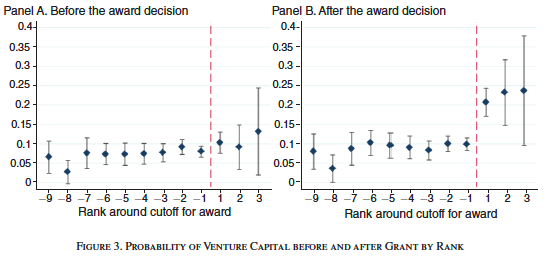
\includegraphics[width=0.8\textwidth, keepaspectratio]{RD_fig.png}
\caption{Reception of venture capital, before and after}
\end{figure}
\end{itemize}
\end{frame}

\begin{frame}
\frametitle{Dell ECMA 2010: Multivariate running variables }
\begin{itemize}
\item Long run effect of extractive institutions on consumption and health outcomes
\begin{figure}[H]
\centering
\includegraphics[width=0.8\textwidth, keepaspectratio]{RD_Dell.png}
\caption{Consumption and Stunting (Darker: less consumption and more stunting)}
\end{figure}
\end{itemize}
\end{frame}



\begin{transitionframe}
  \begin{center}
         { \Huge \textcolor{white}{Machine learning: Gradient descent methods}}
       \end{center}
\end{transitionframe}




\begin{frame}
\frametitle{We worry about model selection for predicting out-samples}
\begin{itemize}
\item In determining the structure, we face the tradeoff between better fit and predictive capabilities of the model (overfitting can be bad for prediction)
\item Model selection: We start with a set $\mathcal{M}$ of candidate models. Then for a model $M\in\mathcal{M}$, we define a penalty parameter $p(M)$ that increases in complexity 
\begin{itemize}
\item Akaike's Information Criterion: Choose $M$ satisfying
\[
\min_{M}\left(\min_\theta\left[ -\sum_{i=1}^n \log{l_i(\theta;M)}+2p(M) \right]\right)
\]
\item Bayesian Information Criterion: Choose $M$ satisfying
\[
\min_{M}\left(\min_\theta\left[ -\sum_{i=1}^n \log{l_i(\theta;M)}+p(M)\frac{\log{n}}{2} \right]\right)
\]
\end{itemize}
\end{itemize}
\end{frame}

\begin{frame}
\frametitle{Penalized optimization}
\begin{itemize}
\item We minimize
\[
\sum_{i=1}^n(Y_i-X_i\theta_0)^2+\lambda\sum_{k=1}^p \theta_k^2 \ \ \left(\sum_{k=1}^p \theta_k^2=\Vert \theta\Vert_2^2\right) \ \ \text{(Ridge)}
\]
Or
\[
\frac{1}{n}\sum_{i=1}^n(Y_i-X_i\theta_0)^2+\lambda\sum_{k=1}^p |\theta_k|   \ \ \text{(LASSO)}
\] 
\item $\lambda$ selected through leave-one-out, $k$-fold cross validation etc. 
\end{itemize}
\end{frame}

\begin{frame}
\frametitle{Classical gradient descent: Newton method}
\begin{itemize}
\item We want to minimize a loss function ($l(\cdot)$ is continuously differentiable in $\theta$)
\[
L(\theta) = \frac{1}{n}\sum_{i=1}^n l(y_i,\theta)
\]
\item By Taylor expansion ($\tilde{\theta}$: Current point, $\theta^{(k)}$, $\theta$: Next point to be reached $\theta^{(k+1)}$)
\[
L(\theta) \simeq L(\tilde{\theta})+L'(\tilde{\theta})(\theta-\tilde{\theta})+\frac{1}{2}L''(\tilde{\theta})(\theta-\tilde{\theta})^2
\]
\item We solve
\[
\frac{d}{d(\theta-\tilde{\theta})} = L'(\tilde{\theta}) + L''(\tilde{\theta})(\theta-\tilde{\theta})=0 \implies  \theta^{(k+1)}= \theta^{(k)}-\frac{L'(\theta^{(k)})}{L''(\theta^{(k)})}
\]
\item Multiple dimensions: $\theta^{(k+1)}= \theta^{(k)}-s_k \nabla L(\theta^{(k)})$ ($s_k$ converges to inverse Hessian matrix at minima and $\nabla L(\cdot)$ is a gradient matrix)
\end{itemize}
\end{frame}


\begin{frame}
\frametitle{Stochastic gradient descent: Useful with large $n$ and $\theta$}
\begin{itemize}
\item With increasing dimensions and observations, we end up doing many more iterations, which can be costly
\item Stochastic gradient descent: Pick a random mini batch of $m$ observations $B_k$ and use the estimate of a gradient from this set of observations to optimize
\item In equation, 
\[
\theta^{(k+1)}= \theta^{(k)}-s_k \frac{1}{m}\sum_{i\in B_k} \nabla_\theta l (y_i, \theta^{(k)})
\]
where $\frac{1}{m}\sum_{i\in B_k} \nabla_\theta l (y_i, \theta^{(k)})$ is the average gradient
\item Additional noise is useful for obtaining global minima that may be far away from local ones (useful in large settings)
\item  The step size $s_k$ decreases as we approach the correct global minima and it is known to give an error in $\frac{1}{\sqrt{k}}$
\end{itemize}
\end{frame}

\begin{frame}
\frametitle{Minibatch gradient descent}
\begin{itemize}
\item It splits the training data into several mini-batches and conducts the optimization on each batch iteratively
\item Procedure
\begin{itemize}
\item Find a minimizer in the first batch $\theta^{(1)}$ from the first batch.
\item Then use $\theta^{(1)}$ as a starting point and use the gradient descent in batch 2 to find a minimal in $\theta^{(2)}$. 
\item Repeat the process until the learning process slows down and we reach a global minima.
\end{itemize}
\item Uses of stochastic gradient: Backbone of artificial neural networks, geophysics, and training of linear models
\end{itemize}
\end{frame}

\begin{frame}
\frametitle{Ensemble method: Combining algorithms for better predictions}
\begin{itemize}
\item Think of ensemble as an average of pre- dictions from multiple sources, with weights determined depending on the performance of the individual algorithms
\item So we solve ($y$ : target, $p_m$ : weight on algorithm $m$, $\hat{y}_m$: prediction from algorithm $m$)
\begin{gather*}
\min_{p_1,..,p_q}L\left( y, \sum_{m=1}^q p_m\hat{y}_m\right) \leq \min_{m\in\{1,..,q\}}L(y,\hat{y}_m)\\
\text{s.t.} \sum_{m=1}^q p_m=1, \ \ p_m\geq0
\end{gather*}
\item Application: Remote sensing and detecting stock price manipulation
\end{itemize}
\end{frame}

\begin{frame}
\frametitle{Gradient boosting: Reduce errors from weak learners with iteration}
\begin{itemize}
\item Imagine having a simple model - regression with few covariates/decision trees with few branches
\item  Our goal is to minimize the prediction error $\sum_{i=1}^n (y_i-\hat{y}_i)^2 $ from the simple models in class $\mathcal{M}$, while penalizing complexity
\item Start with a null predictor $\hat{y}_i^{(0)}=0$ and residuals $r_i^{(0)}=y_i-\hat{y}_i^{(0)}=y_i$. Then:
\begin{enumerate}
\item Fit sample model to data $(x_i, r_i^{(0)} =y_i)$, penalize complexity, and get new predictors $\hat{r}_i^{(1)}$
\item Update the predictions $\hat{y}_i^{(1)}=\hat{y}_i^{(0)}+s\hat{r}_i^{(1)}$
\item Update the residuals $\hat{r}_i^{(1)}=\hat{r}_i^{(0)}-s\hat{r}_i^{(1)}$
\item Iterate for each $b=1,...,B$
\end{enumerate}
\end{itemize}
\end{frame}

\begin{frame}
\frametitle{Gradient boosting: Reduce errors from weak learners with iteration}
\begin{itemize}
\item To conduct the first step in case of parametric models with complexity penalty $p(M)$, choose $M$ and $\theta_M$ that minimizes
\[
\sum_{i=1}^n (r_i^{(b-1)}-r_M(x_i,\theta_M))^2+p(M)
\]
where $\hat{r}^{(b)}=r_M(x_i,\theta_M)$\par
\item  Gradient boosting is used in any fields are the machines are trained to learn to rank (also known as machine-learned ranking) - search engines.
\item  Some physics fields, such as high energy physics, uses this in their data analysis. 

\end{itemize}
\end{frame}


%%%%%%%%%%%
\end{document}
